\documentclass[Main]{subfiles}
\begin{document}

\subsection{Benchmark}

All tests and benchmarks found in this paper, as well as the submitted competition results have been performed on computer with the following specifications:
CPU: 2.3 GHz Intel Core i7 (I7-4850HQ) 
RAM: 8GB allowed to allocate for the client


\textbf{Frontier testing}

As the search is being done, nodes are being added to the frontier. Before a node is added, a check is performed to see if the node already is in the frontier. As the frontier grows large, this check can be expensive to perform. In order to make the lookup faster, experiments were conducted with a queue and a hash set in parallel. The hash set provides information about whether or not a node is already contained in the frontier.


\begin{figure}[h!]
    \centering
    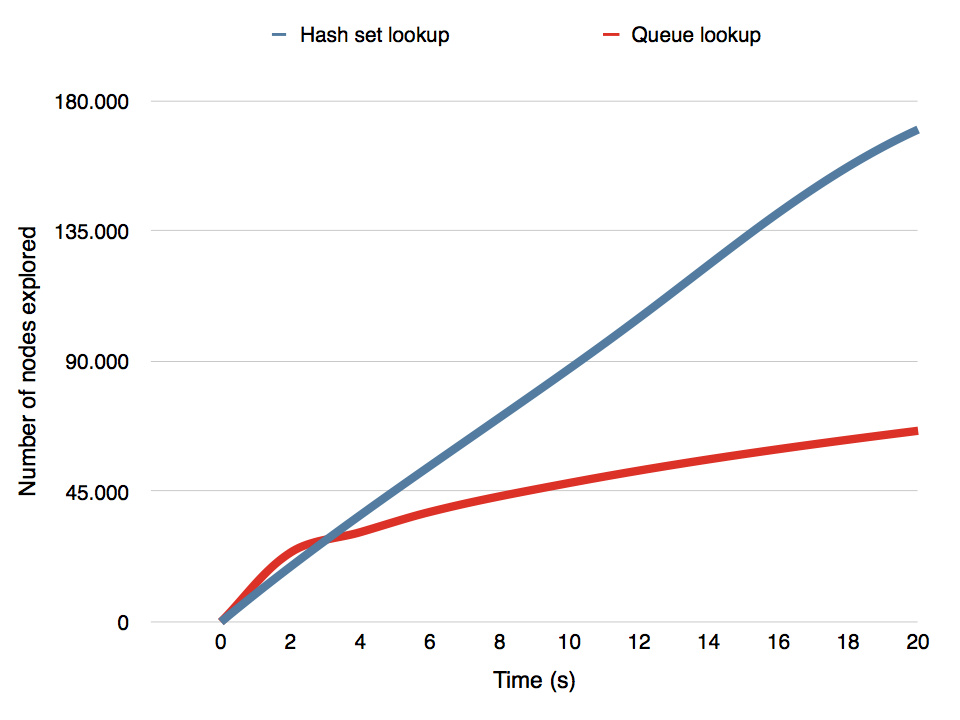
\includegraphics[width=0.3\textwidth]{nodes_explored_compare.png}
    \caption{Comparison of number of nodes explored}
    \label{fig:node_explored_comparison}
\end{figure}

\begin{figure}[h!]
    \centering
    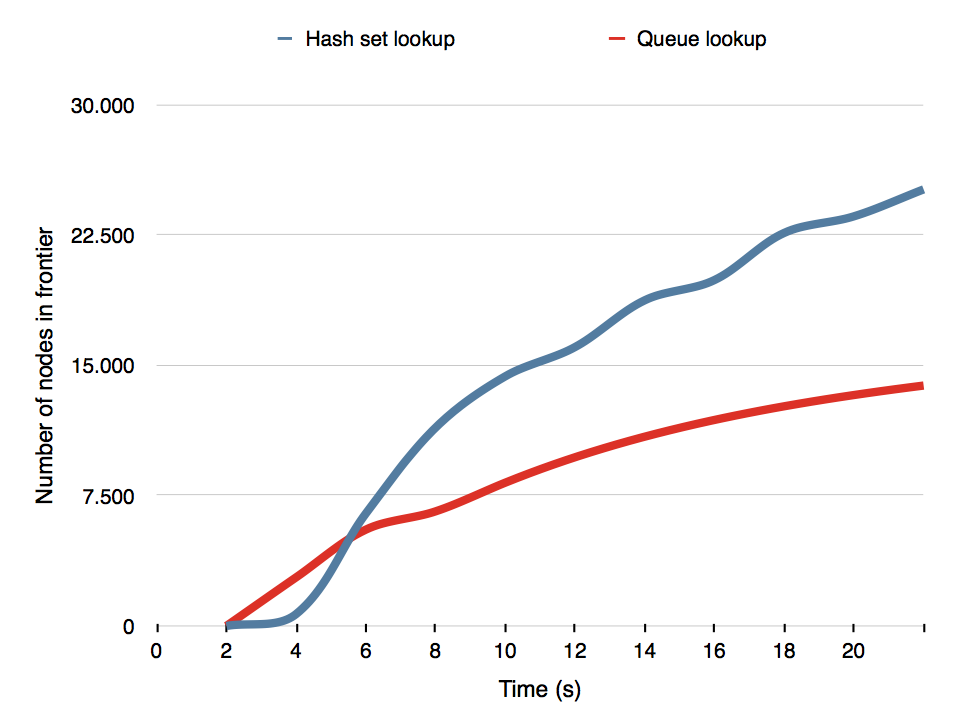
\includegraphics[width=0.3\textwidth]{nodes_in_frontier_compare.png}
    \caption{Comparison of number of nodes in frontier}
    \label{fig:node_frontier_comparison}
\end{figure}


% % % % % % % % % % % % Something


\textbf{Strategy tests}

- Multi vs. single BFS: Should show something about speed versus better solution 



The most interesting experiments conducted with the used search strategy involved two strategies. Best-first search using A* evaluation and a modified version, multi-queue best-first search using A\^{*} evaluation. The strategy applies to both relaxed and full problem search. 
The multi-queue best-first search utilizes two queues, one active ``main queue'' and one ``back-up queue''. The strategy is a very naive implementation of a multi-queue BFS, as a normal implementation alternates between expansions of the nodes in both queues \pcite{hector2013a}, whereas our implementation relies heavily on the ``main queue'' being the \textif{``correct queue''}. Every time a node is expanded, all other nodes in the ``main queue'' are added to the ``back-up queue'' and removed from the main, such that the child nodes from the expanded node are the only nodes in the ``main queue''. In effect this means that our strategy always believes it makes the right choice, which of course is not the case. In the case where the expanded nodes do not lead to solving a goal, the ``main queue'' will at some point turn up empty. When this happens, the most promising node from the ``back-up queue'' is expanded. As the strategy uses A\^{*} evaluation, it is likely that the most promising node will be a node early in the node tree, as its traveled path is short or non-existing. 


The two strategies are compared by comparing the solutions they find to a level. The comparison is regarded from two aspects; completion time, and used actions. 



As the multi-queue BFS implementation functions as a combination of best-first-search and depth-first-search, it could possibly reach a goal state faster than the normal BFS. The found solution could however be much less than optimal. The standard BFS A\^{*} search is more likely to produce a solution that is more optimal than multi-queue BFS, whereas it might spend more time reaching the goal state. 



As an example of a fast, but ``stupid'' solution solution found using the multi-queue BFS strategy, the level SAHoldkaeft is regarded. A solution to the level is found in 1.6 seconds, with an action set consisting of 536 moves. 
The single-queue BFS strategy uses 22.6 seconds to find a solution. The solution is however much shorter at 210 moves. 


% Multi-queue BFS:
% Time: 1603 ms
% Actions: 536

% Single-queue BFS:
% Time: 22642 ms
% Actions: 210




%%%%%%%%%%%%% Move below to queue experimenting

% 20 second run 
% BFS:

% [Client said] Search starting with strategy Best-first Search (PriorityQueue) using A* evaluation
% [Client said] #Explored:    0, #Frontier:   1, Time: 0.00 s     [Used: 291.41 MB, Free: 316.59 MB, Alloc: 608.00 MB, MaxAlloc: 7282.00 MB]

% [Client said] #Explored: 79000, #Frontier: 11774, Time: 20.33 s     [Used: 893.79 MB, Free: 727.21 MB, Alloc: 1621.00 MB, MaxAlloc: 7282.00 MB]

% Multi queue BFS:

% [Client said] Search starting with strategy Multi-Best-first Search (PriorityQueue) using A* evaluation
% [Client said] #Explored:    0, #Frontier:   1, Time: 0.00 s     [Used: 260.84 MB, Free: 219.66 MB, Alloc: 480.50 MB, MaxAlloc: 7282.00 MB]

% [Client said] #Explored: 256978, #Frontier: 198642, Time: 20.47 s   [Used: 4007.45 MB, Free: 1369.05 MB, Alloc: 5376.50 MB, MaxAlloc: 7282.00 MB]


\textbf{Analysis}
From the results it is very clear that the multi queue BFS strategy explores more states than BFS. However, the memory consumption is also a great deal higher. Of course this is mainly due to the size of the frontiers combined, which counts over 10 times more than the BFS strategy. 







% Fixed with hashset for contains() lookup
% [Client said] #Explored: 204000, #Frontier: 6386, Time: 20.37 s     [Used: 2111.79 MB, Free: 887.71 MB, Alloc: 2999.50 MB, MaxAlloc: 7282.00 MB]

% [Client said] #Explored: 169000, #Frontier: 5760, Time: 20.94 s  [Used: 1689.85 MB, Free: 1242.15 MB, Alloc: 2932.00 MB, MaxAlloc: 7282.00 MB]




\end{document}


